\documentclass[a4paper,thmnumbering=section,eqnumbering=section]{summary-ja}

\newcommand{\gl}{\textrm{GL}}
\newcommand{\edm}{\textrm{End}}
\newcommand{\reg}{\textrm{reg}}
\newcommand{\hs}{\hspace{1pt}}
\begin{document}
a

\begin{align}
    \Mod\\
    \lnapprox\\
    \left\{a\overrightarrow{a} \right\} \bigotimes \otimes\oplus \bigoplus\amalg \prod \coprod \subseteq \supseteq \succeq \preceq \\
    \blacktriangleleft \blacktriangleright\\
    \neq \subsetneq, \supsetneq, \hookrightarrow, \circlearrowright, \\
    \partial \nabla \infty \ldots \ddots \cdots \vdots \Re \forall \exists \nexists\\
    \varnothing \varnothing \emptyset\wp\\
    \cong \approx \sim \simeq \leq \geq \leqslant \geqslant \\
    \nprec \Longleftarrow \Longrightarrow \Rightarrow \Leftarrow \longleftarrow \longrightarrow \longmapsto \\
    \surd \dagger \binom{e}{f} \\
    \left\langle \right\rangle \left\lfloor \right\rfloor \\
    \oint \iint 
\end{align}
\noindent
これは\(\Set\)\\
これは\(\Top\)\\
これは$\Grp$\\
これは$\Ab$\\
これは$\Cring$\\
これは$\Ring$\\
これは$\Rng$\\
これは$\Sch$\\
これは$\Mod$\\
これは$\Coh$\\
これは$\QCoh$


\begin{myproof}
    aaa証明
\end{myproof}
\begin{myproof}
    aaa証明\\
    どうなの？それは
\end{myproof}





\tableofcontents
\setcounter{section}{-1}

\newpage\section{予備知識}% section 0 ==============================================================================================================
\begin{definition}{群}{}
    群$G$とは，...
\end{definition}

\begin{definition}{環}{}
    環とは，...
\end{definition}

ここでは以後，環は全て可換とは限らない単位的なものであるとし，環の射は単位元を保つものとする．
\begin{definition}{加群}{}
    アーベル群$M$は，環$R$によるスカラー作用，すなわち...
\end{definition}

\begin{definition}{自由$R$加群}{}
    $R$加群$M$が自由であるとは，ある集合$I$があって，$M$が$R$の直和加群$R^{\oplus I}$に同型となることをいう．
\end{definition}

\begin{definition}{群環}{}
    $R$を環，$G$を群とする．$G$上の自由$R$-加群$R[G]$には，次のようにして積の構造が定まる；
    \begin{align}
        a = \sum_{x\in G}{}a_xx, \; b = \sum_{x\in G}{}b_xx \text{ に対し，}
        ab \coloneqq \sum_{x\in G}{}\sum_{\substack{u,v\in G \\ uv=x} }{}a_ub_vuv
    \end{align}
    このようにして新たに得られる環としての$R[G]$を，\textbf{$G$の$R$上の群環(group ring of $G$ over $R$)}という．
\end{definition}

\begin{definition}{作用}{}
    $G$を群，$X$を集合とする．$G$の$X$に対する\textbf{作用}とは，$X$上の可逆な変換のなす群を$\textrm{Aut}(X)$として，
    群準同型$G\ri \textrm{Aut}(X)$のことをいう．
\end{definition}
% ========================================================================================================================



\newpage\section{表現の定義}% section 1 ==============================================================================================================

ここでは，群の（有限次元）表現に関する一般的な定義と結果を与える．有限群に特有の
結果については，のちの章で詳しく考察する．
\begin{definition}{表現とその射}{}\par
    \quad \textbf{$G$の($k$上の)表現(representation of $G$ over $k$)}とは，
    $k$-ベクトル空間$V$と， $G$から$\gl(V)$への群準同型写像$\rho$の対
    $(V,\rho)$のことであり，このとき$V$を表現$(V,\rho)$の
    \textbf{表現空間(representation space of $G$)}，
    $\dim_k(V)$を\textbf{表現の次元(dimension of representation)}という．
    また，表現空間としてベクトル空間$V$を持つような$G$の表現をとくに
    \textbf{$V$上の表現(representation on $V$)}という．\par
    \quad $G$の表現$(V,\rho_V),(W, \rho_W)$に対し， $k$-準同型$\varphi:V\ri W$が
    $(V,\rho_V)$から$(W, \rho_W)$への\textbf{表現の射(morphism of representations)}
    あるいは\textbf{$G$-準同型($G$-morphism)}であるとは，
    任意の$g\in G$に対して以下の図式が可換になることをいう；
    \begin{align}
        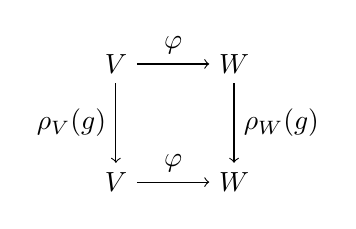
\begin{tikzpicture}
            \node (Vup) at (0,0) {$V$};
            \node (Wup) at (1.5,0) {$W$};
            \node (Vdown) at (0,-1.5) {$V$};
            \node (Wdown) at (1.5,-1.5) {$W$};
            \draw[->] (Vup) -- node[above] {$\varphi$}  (Wup); 
            \draw[->] (Vup) -- node[left] {$\rho_V(g)$} (Vdown);
            \draw[->] (Wup) -- node[right] {$\rho_W(g)$} (Wdown);
            \draw[->] (Vdown) -- node[above] {$\varphi$} (Wdown);
            \node at (0.7,-0.7) {$\circlearrowright $};
        \end{tikzpicture}
    \end{align}
    \quad 表現の射$\varphi$に対して， $\Ker\hs\varphi, \Im\hs\varphi, \Coker\hs\varphi$
    は全て$k$-準同型のときと同様に定義する．
    また$(W, \rho_W)$から$(V,\rho_V)$への$G$-準同型$\psi$が
    $\psi\circ\varphi=\id_{V},\hs \varphi\circ\psi=\id_{W}$を満たすものが存在する
    とき$\varphi$は\textbf{同型射(isomorphism)}であるといい，
    $(V,\rho_V)$と$(W, \rho_W)$は\textbf{同値な表現(equivalent representation)}であるという．\par
    \quad 以後， $G$の表現$(V,\rho)$や$g\in G$の$\rho$による像$\rho(g)$をそれぞれ，
    単に$V$或いは$\rho$や， $g$などと書くことがある．
\end{definition}

\begin{remark}
    $G$の表現$(V,\rho)$によって，表現空間$V$を群環$k[G]$上の加群と見なすことができる．
    これは，各$\sum_{g\in G} a_gg\in k[G]$と$v\in V$に対して，
    $(\sum_{g\in G} a_gg) v = \sum_{g\in G} a_g\rho(g)(v)$
    とすれば良い．
\end{remark}

\begin{remark}
    $G$の$V$上の表現を与えることは， $G$の$V$への左作用を与えることと同じである．したがって
    表現$(V,\rho)$において， $\rho$は$G$の$V$への左作用を与えている．
\end{remark}

\begin{example}{自明表現}{自明表現}
    $G$を群， $V$を任意の$k$ベクトル空間とする．群準同型
    $\mathbf{1}_G:G\ni g \longmapsto \id_{V}\in \gl(V)\; (\forall g\in G)$
    によって定まる$G$の表現$(V,\mathbf{1}_G)$を，$G$の\textbf{自明表現(trivial representation)}
    という．自明表現は，ベクトル空間$V$の取り方によらず全て同値である．
\end{example}

\begin{example}{行列式が定める表現}{行列式表現}
    群として$GL_n(k)(k\text{上の}n\text{次一般線型群})$をとると，
    $(k, \det)$は$GL_n(k)$の一次元表現である．
\end{example}


\begin{example}{有限群の正則表現}{有限群の正則表現}
    有限群$G$に対し， $G$の元によって生成される体$K$上の自由ベクトル空間を$V_{\text{reg}}$とする；
    $V_{\text{reg}}=\bigoplus_{x\in G}Kx$．（これは，$G$の$K$上の
    群環$K[G]$から積を忘れたものと同じである）．また$\rho_{\reg}:G\ri \gl(V_{\reg})$を，
    各$g\in G$と$x\in G$に対して
    $\rho_{\reg}(g)(x) = gx$と定めると， $(V_\reg, \rho_\reg)$は$G$の表現である．
    これを$G$の\textbf{正則表現(regular representation)}といい， $R_G$や$R$などと表す．
\end{example}


\begin{example}{表現のテンソル積・直和}{テンソル積・直和}
    $(V,\rho_V),(W,\rho_W)$を$G$の$k$上の二つの表現とする．
    $V,W$の\textbf{テンソル積表現}とは，
    $V$と$W$の$k$上のテンソル積$V\otimes_kW$を表現空間とし，
    $V\otimes_kW$への作用$\rho_V\otimes\rho_W$を，各$g\in G$に対して
    $\left( \rho_V\otimes\rho_W \right)(g) \coloneqq \rho_V(g)\otimes \rho_W(g)$
    （線型写像のテンソル積）として定めたもの$(V\otimes_kW, \rho_V\otimes\rho_W)$
    である．表現の直和も同様にして定まる．
\end{example}

\begin{example}{双対表現}{双対表現}
    $G$の表現$(V,\rho)$に対して，表現空間を$V$の双対空間$V^\ast=\text{Hom}_k(V,k)$，
    $V^\ast$への作用$\rho^\ast$を，各$g\in G$に対して
    $\rho^\ast (g) = (\rho(g^{-1}))^\ast:V^\ast \ni \alpha \longmapsto \alpha \circ \rho(g^{-1}) \in V^\ast $
    によって定めた表現$(V^\ast, \rho^\ast)$を， $(V,\rho)$の\textbf{双対表現(dual representation)}
    という．
\end{example}

\begin{definition}{部分表現・既約表現}{既約表現}
    $(V,\rho)$を$G$の表現とする．$V$の$k$-部分空間$V^\prime$が$G$の作用で閉じている，すなわち
    \[ G V^\prime \subseteq V^\prime \Longleftrightarrow 
    \; gv \in V^\prime \; \left(\forall g\in G, \forall v\in V^\prime\right)\]
    を満たすとき，$V^\prime$を$V$の\textbf{$G$-不変部分空間}あるいは\textbf{$G$部分空間}という．
    $V^\prime$が$V$の$G$部分空間であるとき，各$g\in G$に対して，$g|_{V^\prime}$は
    $V^\prime$上の可逆な線型変換を誘導し，これによって定まる
    $V^\prime$への作用を$\rho_{V^\prime}$と記すと，$(V^\prime, \rho|_{V^\prime})$は$G$の表現となる．
    このようにして，$V$の$G$不変部分空間によって与えられる表現を$V$の\textbf{部分表現}という．\par
    \quad$V$が自明な$G$部分空間しか持たないとき，
    $V$は\textbf{既約(irreducible)}であるという．そうでないときは$V$は
    \textbf{可約(reducible)}であるといい，$V$の部分表現で既約なものを$V$の\textbf{既約成分(irreducible component)}という．
    
\end{definition}

\begin{example}{対称群の置換表現}{置換表現}
    $n$次対称群$\mathfrak{S}_n$の$k^n$上の表現を考える．
    $k^n$の標準基底$(e_1, \cdots, e_n)$によって， $\gl(k^n)$と$k$上の$n$次一般線型群
    $GL_n(k)$とを同一視する．
    $\mathfrak{S}_n$の$k^n$への作用$\rho$を，各$\sigma\in\mathfrak{S}_n$に対して
    $\rho(\sigma)= E_\sigma = [\delta_{i\sigma(j)}]_{1\leq i,j\leq n}$
    （つまり， $E_\sigma$は各$e_i$を$e_{\sigma(i)}$へ移すような線型変換である）と定める
    ことにより得られる表現$(k^n, \rho)$を， $n$次対称群$\mathfrak{S}_n$の\textbf{置換表現}という．
    各$x=(x_1, \cdots, x_n)\in k^n$に対して
    $E_\sigma(x) = (x_{\sigma^{-1}(1)}, \cdots, x_{\sigma^{-1}(n)})$
    となる．そこで$k^n$の$(n-1)$次元部分空間$H$を$H=\{ x\in k^n \;|\; \sum_i x_i = 0\}$とすると
    これは置換表現の真の部分表現を与えている．したがって，一般に$n$次対称群の置換表現は可約である．
\end{example}

\begin{example}{Hom表現}{Hom表現}
    $G$の表現$(V,\rho_V), (W,\rho_W)$に対して，$G$の$\Hom_k(V,W)$への表現を次のように定める；
    \begin{center}
        各$g\in G$と$\varphi\in\Hom_k(V,W)$に対し，\vspace{-10pt}
        \begin{align}
            \rho_{\textrm{Hom}}(g)(\varphi) \coloneqq \rho_W(g)\circ\varphi\circ\rho_V(g^{-1}).
        \end{align}
    \end{center}
    すると，これは$W$と$V$の双対表現$V^\ast$とのテンソル積表現に同値である．

\end{example}

\begin{remark}
    $G$-morphism $\varphi:V\ri W$に対して，
    $\Ker\hs\varphi, \Im\hs\varphi$はそれぞれ$V,W$の部分表現を与える．
\end{remark}

\begin{theorem}{Schurの補題}{シューアの補題}
    \quad $G$を任意の群，$k$は任意の代数閉体であるとし，$V,W$をともに$G$の既約表現とする．このとき，
    $k$ベクトル空間としての同型
    \begin{align}
        \Hom_G(V,W) \cong_k
            \begin{cases}
                k & (  V\cong_G W) \\
                0 & (  V\not\cong_G W)\\
            \end{cases}
    \end{align}
    が成り立つ．とくに，$V=W$の場合は同型は$k$代数としての同型となる．
\end{theorem}
\begin{myproof}\par
    [$V=W$のとき]\quad
    任意の$\varphi\in\edm_G(V)=\Hom_G(V,V)$は$k$に固有値$\lambda$を
    もち，その固有空間$\Ker\hs(\varphi - \lambda\hs\id_V)$は$G$不変部分空間である．
    $V$が既約であることから$\varphi=\lambda\hs\id_V$が成り立ち，これによって
    写像\[\edm_k(V)\ni\varphi\longmapsto(\varphi\textrm{の固有値})\in k\]が定まる．
    これは明らかに$k$代数の同型を与えている．\par
    [$V\cong_G W$のとき]\quad
    $f:W\ri V$を$G$同型とすると，$k$準同型
    \[\Hom_G(V,W) \ni \varphi \longmapsto f\circ\varphi\in \edm_k(V)\]
    が定まり，これが同型であることは容易に確認できる．\par 
    [$V\not\cong_G W$のとき]\quad
    $\varphi\in \Hom_G(V,W)$が$\varphi\neq 0$とすると，
    $\Ker\hs\varphi=0$かつ$\Im\hs\varphi = W$が成り立つので$\varphi$は同型となり，仮定に矛盾する．
\end{myproof}
% ========================================================================================================================


\newpage\section{有限群の表現の基本定理}% section 2 ==========================================================================================

\begin{definition}{不変直和因子，完全可約性}{}
    $G$を任意の群，$V$をその表現とする．$V$の部分表現$V^\prime$は，
    ある$V$の部分表現$V^{\prime\prime}$が存在して，表現としての直和
    $V\cong V^\prime\oplus V^{\prime\prime}$を満たすとき，$V$の\textbf{不変直和因子}であるという．
    また$V$は，その既約成分の直和として表されるとき\textbf{完全可約}であるという．
\end{definition}

\vspace{1em}一般に群$G$の表現$V$に対して，部分表現は不変直和因子となるとは限らない．
実際，群$G$として$\ZZ$をとり，$\ZZ$の$\CC^2$への表現を
\[
    \ZZ \ni a \longmapsto 
    \begin{bmatrix}
        1 & a \\
        0 & 1 \\
    \end{bmatrix} \in GL_2(\CC)
\]によって定めると，
$\left\{
    (x,0) \;\middle|\; x\in \CC
\right\} = \CC e_1 \subsetneq  \CC^2$は$\ZZ$-invariant space を与える．
他方，どのような補空間をとっても，直和因子となることはない．\par
しかし，有限群$G$の表現を考える上では，"直和因子"という概念と"$G$不変空間"という概念が一致するのである．
このことを示しているのが次の定理である．
\begin{theorem}{Mascheの定理}{Masche}
    $k$を任意の体とする．有限群$G$の$k$じょうお
    $G$を有限群とする．
    $|G|$が
\end{theorem}

\begin{lemma}{完全可約性の特徴づけ}{完全可約性の特徴づけ}\quad
    $G$は任意の群，$V$を任意の体$k$上の$G$の有限次元表現とする．
    $V$が完全可約であるためには，$V$の任意の部分表現$W$に対して，
    $V\cong W\hspace{-1pt}\oplus U$となるような部分表現$U$が存在することが必要十分である．
\end{lemma}\vspace{-1em}
\begin{myproof} \color{red}{まず，$V$の有限次元性から，$V$の直和因子は（存在すれば）有限個であることに注意する．$\dim_k V$による
    帰納法によって示す．\par 
    まず$V$が完全可約で，既約成分$V_1,\cdots, V_r$によって
    $V \cong V_1 \oplus \cdots \oplus V_r$と表せるとする．$\dim_k =1$のときには明らかである．$\dim_k V>1$として，
    $W$を$V$の自明でない部分表現とする．このとき
    $(W\cap V_1) \oplus \cdots \oplus (W\cap V_r)$は$W$の直和分解であり，}
\end{myproof}


\begin{theorem}{Mascheの定理}{}
    $G$を有限群で，その位数$|G|$は$k$の標数$p$を割り切らないとする．
\end{theorem}
ましゅましゅマーシュ
\begin{myproof}
    aaa??
\end{myproof}


\end{document}